\documentclass[border=10pt]{standalone}
\usepackage[svgnames]{xcolor}
\usepackage{amsmath}
\usepackage{pgfplots}
\pgfplotsset{compat=newest}
\usepackage[sfdefault]{FiraSans}
\usepackage{FiraMono}
\renewcommand*\familydefault{\sfdefault}
\begin{document}
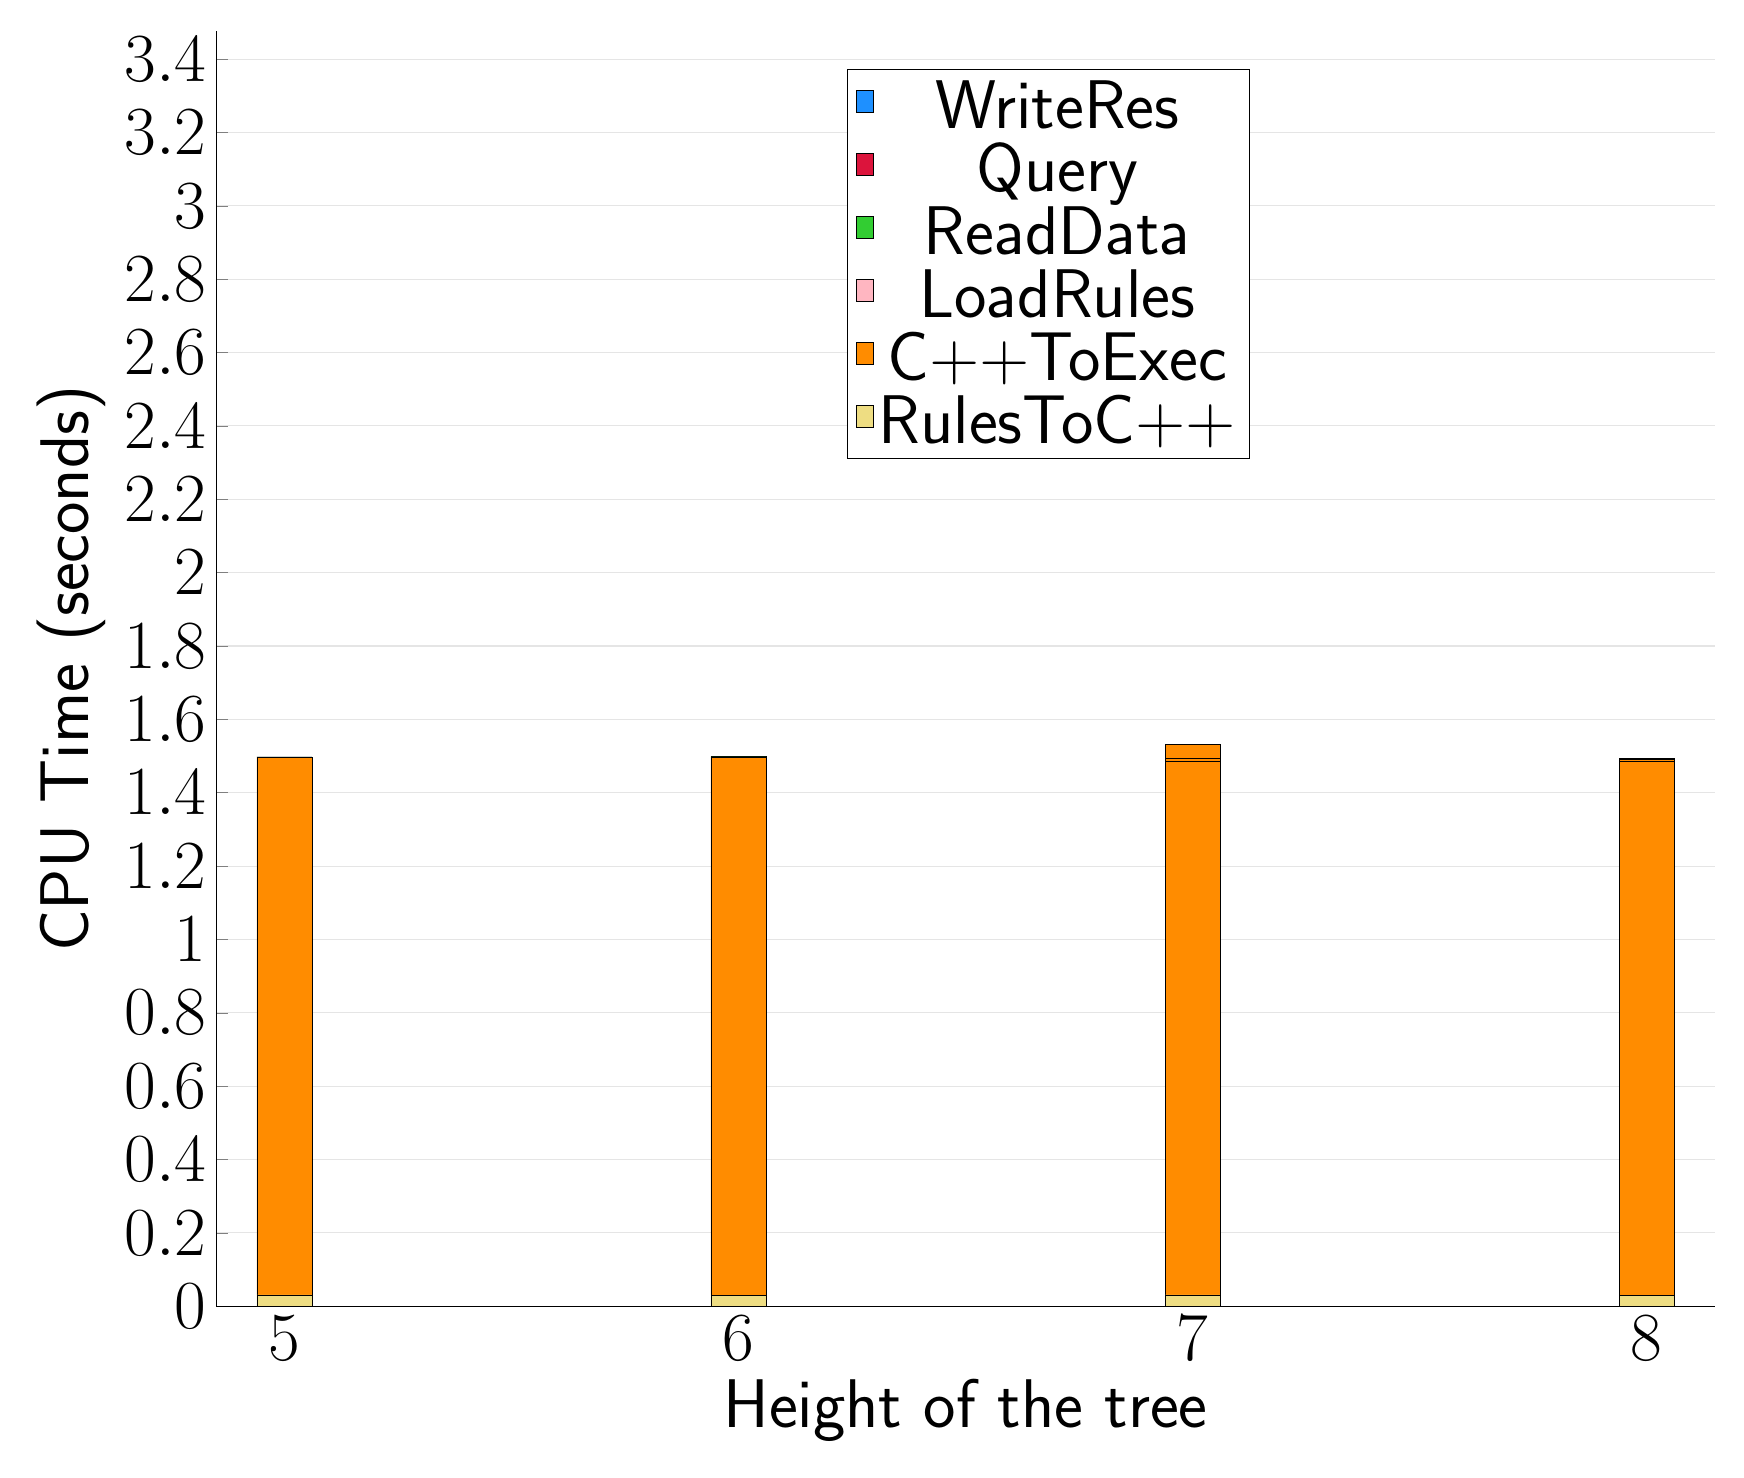
\begin{tikzpicture}
	\begin{axis}[
			ybar stacked,
			width=1.7\textwidth,
			bar width=0.7cm,
			ymajorgrids, tick align=inside,
			major grid style={draw=gray!20},
			xtick=data,
			ymin=0, ymax=3.477,
			axis x line*=bottom,
			axis y line*=left,
			enlarge x limits=0.05,
			legend style={
					at={(0.69, 0.97)},
					anchor=north east,
					legend columns=1,
					font=\Huge,
				},
			ylabel={CPU Time (seconds)},
			xlabel={Height of the tree},
			label style={font=\Huge},
			tick label style={font=\Huge},
		]
		\addlegendimage{fill=DodgerBlue, draw=black, line width=0.2pt}
		\addlegendentry{WriteRes}
		\addlegendimage{fill=Crimson, draw=black, line width=0.2pt}
		\addlegendentry{Query}
		\addlegendimage{fill=LimeGreen, draw=black, line width=0.2pt}
		\addlegendentry{ReadData}
		\addlegendimage{fill=LightPink, draw=black, line width=0.2pt}
		\addlegendentry{LoadRules}
		\addlegendimage{fill=DarkOrange, draw=black, line width=0.2pt}
		\addlegendentry{C++ToExec}
		\addlegendimage{fill=LightGoldenrod, draw=black, line width=0.2pt}
		\addlegendentry{RulesToC++}
		\addplot +[fill=LightGoldenrod, draw=black, line width=0.2pt] coordinates {
				(5, 0.031000000000000007)
				(6, 0.030000000000000006)
				(7, 0.030000000000000006)
				(7, 0.031000000000000007)
				(7, 0.030000000000000006)
				(8, 0.030000000000000006)
				(8, 0.030000000000000006)
				(8, 0.030000000000000006)
			};
		\addplot +[fill=DarkOrange, draw=black, line width=0.2pt] coordinates {
				(5, 1.466)
				(6, 1.467)
				(7, 1.501)
				(7, 1.4629999999999999)
				(7, 1.4569999999999996)
				(8, 1.4549999999999998)
				(8, 1.4600000000000002)
				(8, 1.4599999999999997)
			};
		\addplot +[fill=LightPink, draw=black, line width=0.2pt] coordinates {
				(5, 0.00012030000000000001)
				(6, 0.00013050000000000003)
				(7, 8.26e-05)
				(7, 9.44e-05)
				(7, 0.00012029999999999998)
				(8, 9.72e-05)
				(8, 9.859999999999998e-05)
				(8, 0.0001232)
			};
		\addplot +[fill=LimeGreen, draw=black, line width=0.2pt] coordinates {
				(5, 0.0003086)
				(6, 0.00043560000000000007)
				(7, 0.00047410000000000003)
				(7, 0.00046879999999999996)
				(7, 0.0005165)
				(8, 0.0007673999999999999)
				(8, 0.000788)
				(8, 0.0008012999999999999)
			};
		\addplot +[fill=Crimson, draw=black, line width=0.2pt] coordinates {
				(5, 0.00013099999999999999)
				(6, 0.00037610000000000003)
				(7, 0.0007089999999999999)
				(7, 0.0006937)
				(7, 0.0007836)
				(8, 0.0018126999999999998)
				(8, 0.0018664)
				(8, 0.0019291)
			};
		\addplot +[fill=DodgerBlue, draw=black, line width=0.2pt] coordinates {
				(5, 0.0002651)
				(6, 0.00039779999999999997)
				(7, 0.0004694)
				(7, 0.0004426)
				(7, 0.0005087)
				(8, 0.0009031000000000001)
				(8, 0.0009285)
				(8, 0.000932)
			};
	\end{axis}
\end{tikzpicture}

\end{document}
